\scanpage{25}
\begin{flushright}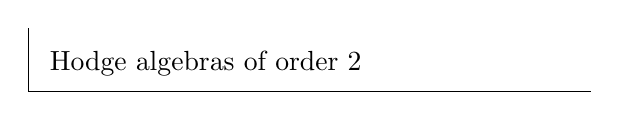
\begin{tikzpicture}
\node[anchor=west] at (0,0) {Hodge algebras of order 2};
\draw (-.15,.45)--(-.15,-.35)--(7,-.35);
\end{tikzpicture}\end{flushright}
\diagram{\begin{array}{ccccc}
H^0&H^1&H^2&H^3&H^4\\
k&V&k\xi+W&\check V&k\xi^2
\end{array}}

$V,W$

\[
\bigwedge^2 V\xrightarrow{\alpha}k\xi+W
\qquad \alpha(x\wedge y)=\varphi(x,y)\xi+\psi(x,y)
\]
\[
\operatorname{Sym}^2(W)\xrightarrow{\beta}k\xi^2
\qquad \beta(xy)=Q(x,y)\xi^2
\]
\margin{$\varphi(x,y)$ alternating form\par
$\psi(x,y)$ -- alternating bilinear map into $W$\par
$Q$ symmetric bilinear form on $W$}

\deleted{\unsure{Point of view}}
Knowledge of $V,W,\varphi,\psi,\bar Q$ makes it possible to reconstruct $H^*$ :
up to canonical isomorphism.

\[
H^0\times H^i\longrightarrow H^i:\quad\text{clear from}\quad
1.x=x.1=x\qquad\forall x.
\]
\[
H^1\times H^i\longrightarrow H^{i+1}\quad
\left|\begin{array}{ll}
\deleted{\unsure{therefore|of which}}\ i=1&xy=\varphi(x,y)\xi+\psi(x,y)\qquad x,y\in V\\
i=2&\begin{array}{l}
x\xi=\xi x=\widetilde\varphi(x):\quad\deleted{\unsure{(*)}}\ y\longmapsto\varphi(y,x)\\
xw=wx=\rho(w,x):\quad y\longmapsto Q(\psi(y,x),w)
\end{array}\quad\left|\begin{array}{l}x\in V\\y\in V\\w\in W\end{array}\right.\\
i=3&xy'=-y'x=\deleted{\unsure{+|-}}\langle x,y'\rangle\xi^2\qquad x\in V,y'\in\check V\\
\deleted{i=4}&\deleted{x\xi^2=0}
\end{array}\right.
\]
\[
H^2\times H^i\longrightarrow H^{j+2}\quad
\left|\quad j=2:\quad\left|\begin{array}{l}
\xi.\xi=\xi^2\\
\xi w=w\xi=0\quad(w\in W)\\
ww'=Q(w,w')\xi^2
\end{array}\right.\right.
\]
\figure{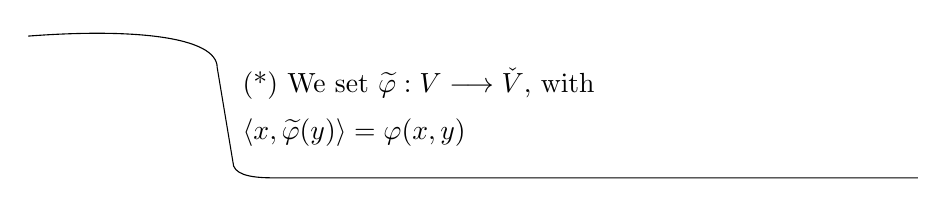
\begin{tikzpicture}[x=1cm,y=1cm]
\node[anchor=west,align=left] at (.2,0) {(*) We set $\widetilde\varphi:V\longrightarrow\check V$, with\\[.5em]$\langle x,\widetilde\varphi(y)\rangle=\varphi(x,y)$};
\draw (-2.4,.9) .. controls (-1.1,1) and (0,.9) .. (0,.5) -- (.2,-.7) .. controls (.2,-.85) and (.4,-.9) .. (.7,-.9) -- (8.9,-.9);
\end{tikzpicture}}

Whatever the choices of $\varphi,\psi$, one finds an anticommutative law of composition,
admitting $1$ as unit.

\uline{Associativity condition} is written $(xy)(tz)=(tx)(yz)$, in the form
\figure{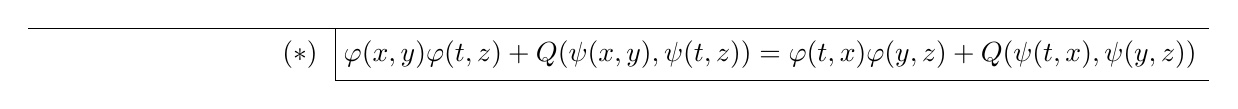
\begin{tikzpicture}
\node[anchor=west,inner sep=0pt] (e) at (0,0) {$\displaystyle\varphi(x,y)\varphi(t,z)+Q(\psi(x,y),\psi(t,z))=\varphi(t,x)\varphi(y,z)+Q(\psi(t,x),\psi(y,z))$};
\node[anchor=east] at (-0.2,0) {$\deleted{\unsure{(*)}}$};
\draw ([xshift=-4cm,yshift=.15cm]e.north west)--([xshift=.15cm,yshift=.15cm]e.north east);
\draw ([xshift=-.1cm,yshift=.15cm]e.north west)--([xshift=-.1cm,yshift=-.15cm]e.south west)--([xshift=.15cm,yshift=-.15cm]e.south east);
\end{tikzpicture}}
\margin{also expresses that the form $(xy)(zt)$ in $xyzt$ is alternating in $y,z$
(hence in \unsure{all the variables!|all the variables!})}

\uline{Lefschetz condition}
\[
\xi^2:H^0\simeq H^4\qquad\text{always satisfied}
\]
\[
\xi:H^1\longrightarrow H^3\qquad\text{if and only if}\quad
\boxed{\varphi\text{ nondegenerate}}
\]

\uline{Poincaré condition}
\[
\begin{array}{l}
H^4\simeq k\quad\text{always satisfied}\\
H^0\times H^4\longrightarrow H^4\text{ and }H^1\times H^3\longrightarrow H^4\quad\text{nondegenerate: }\uline{\text{ditto}}\\
H^2\times H^2\longrightarrow H^4\quad\text{nondegenerate if and only if}\quad\boxed{Q\text{ nondegenerate}}
\end{array}
\]
\mspage{24}
